\chapter{Introdução}
\label{cap:introducao}
Considerado como ponto chave para a Web Semântica \cite{berners2001semantic}, Dados Conectados vem sendo abordado de forma crescente por acadêmicos, governos e empresas. Tal crescimento se deve ao fato de Dados Conectados ser uma alternativa relevante para conectar bases de dados distribuídas na Web. Segundo \citeonline{hyland2011joy}, Dados Conectados se trata de um conjunto de boas práticas para publicar e conectar dados estruturados na Web. Ademais, \citeonline{berners2006linked} afirma que não se trata apenas de por dados na Web, mas fazer conexões entre eles, permitindo assim, que pessoas ou máquinas possam explorar a Web dos dados.

Web de Dados bem como Web dos Documentos, são termos utilizados para descrever o paradigma da Web atualmente, onde o primeiro, que tem como base o segundo, reflete a possibilidade de conectar os dados através de links. Sendo esta, uma possibilidade inexistente quando se fala de Web dos Documentos, pois nesta, os documentos apontam para outros documentos através de links.

Dados Conectados pode ser visto sob duas perspectivas: consumo e publicação. A primeira aborda o ponto de vista do consumidor, tratando a exploração de dados para tornar as aplicações mais ricas. A segunda está sob a perspectiva do publicador, abordando processos \cite{bizer2007publish, hyland2011joy, villazon2011methodological, Avila2015} e conceitos \cite{berners2006linked, wood2014linked} necessários para publicar e manter os dados na Web de forma conectada. 

Publicar ou manter dados conectados na Web vai além de disponibilizar conjuntos de dados através de serializações RDF. É necessário conectá-los a outros conjuntos de dados já existentes. Porém, criar links entre conjuntos de dados requer uma análise cuidadosa por parte do especialista, que apesar de ser uma abordagem eficaz, não é escalável, visto que a quantidade de dados publicados cresce constantemente. Consequentemente, inviabilizando o processo de publicação de forma artesanal. Logo, para que seja possível construir a Web de Dados de forma eficiente, é necessário que existam soluções capazes de conectar dados de forma automática ou semiautomática.

Conectar dados automaticamente é um problema reconhecido por diversas comunidades. Dentre essas comunidades, podemos destacar as comunidades de Bancos de Dados e Web Semântica. Na primeira, esse problema é conhecido através do termo \textbf{\textit{Record Linkage}} \cite{gu2003record}. Na segunda, ele é reconhecido pelo termo \textbf{\textit{Instance Matching}}. Além disso, também é possível encontrar referências como \textbf{\textit{Problema de Resolução de Entidades}} \cite{menestrina2005generic} e \textbf{\textit{Deduplicação}} \cite{sarawagi2002interactive}, que se trata de um processo que tem como objetivo identificar e conectar recursos julgados representar a mesma entidade do mundo real.

Para identificar e conectar recursos na Web, a comunidade vem apresentando um número crescente de soluções (ver Figura \ref{fig:oaei_imtools}). Com o objetivo de avaliá-las, a \textit{Ontology Alignment Evaluation Initiative} (OAEI) realiza uma avaliação anual, que consiste em alinhar dois conjuntos de dados pré-definidos e comparar o alinhamento gerado pela solução com o alinhamento de referência. A partir da comparação entre os dois conjuntos de alinhamento as métricas de precision, recall e f-measure são geradas.

\begin{figure}[!ht]
	\centering
	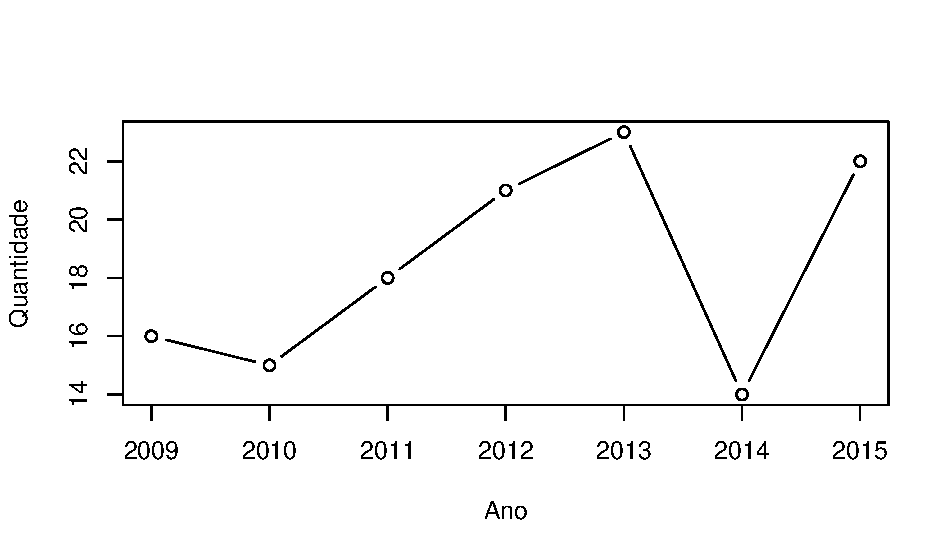
\includegraphics[width=1\textwidth]{./imagens/im_tools.pdf}
    \caption{Quantidade de soluções submetidas ao OAEI}
	\footnotesize{Fonte: \cite{cheatham2015results}.}
	\label{fig:oaei_imtools}
\end{figure}

Porém, de acordo com \citeonline{homoceanu2014putting}, apesar dos bons resultados apresentados, as soluções não estão prontas para alinhar dados automaticamente de forma confiável. Para isso, foi realizado um experimento equivalente ao executado pela OAEI. Entretanto, utilizando dados reais, que foram obtidos de 5 fontes diferentes (Freebase, DBPedia, LinkedMDB, DrungBase e NewYork Times). Além disso, o experimento permitiu notar que não era provido o suporte adequado a algumas propriedades dos vocabulários utilizados.
	
Dentre as propriedades com suporte inadequado, destaca-se a propriedade owl:sameAs, que é responsável por identificar recursos equivalentes. Além disso, essa se trata de uma propriedade transitiva. Dessa forma, se existem dois recursos equivalentes R1 e R2 e existe um terceiro recurso R3 que é equivalente a R2, então R1 é equivalente a R3. Como representado na Figura \ref{sameAs}.Tais características fazem com que a propriedade owl:sameAs seja uma das  mais utilizadas para alinhar dados na Web. Dessa forma, utilizar ferramentas que levem em consideração as características das propriedades é de grande importância para alinhar dados de forma confiável.

\begin{figure}[h]
\centering
\begin{tikzpicture}[node distance=1cm, auto,]
 %nodes
 \node[ellipse,draw] (r3) {R3};
 
 \node[above=of r3] (dummy) {};
 \node[right= of dummy,ellipse,draw](r2) {R2}
 	edge[pil,<->, bend left=45] node[auto] {owl:sameAs} (r3);
 
 \node[left= of dummy,ellipse,draw] (r1) {R1}
  	edge[dashed,<->, bend right=45] node[auto] {owl:sameAs} (r3)
   	edge[pil,<->, bend left=45] node[auto] {owl:sameAs} (r2);
\end{tikzpicture}
\caption{Transitividade da propriedade owl:sameAs}
\label{sameAs}
\end{figure}

Neste contexto, este trabalho propõe uma abordagem independente de contexto para o alinhamento de dados conectados por meio de um processo de alinhamento que leva em consideração aspectos dos dados e  características do modelo ontológico. Assim, os recursos/instâncias analisados, além de alinhados através das propriedades de dados, podem ser alinhados través seus relacionamentos. Ademais, a proposta trata o problema do alinhamento entre datasets reais, permitindo que seja possível alinhar datasets distribuídos na Web de forma confiável.
\subsection*{Objetivo}

Essa abordagem visa disponibilizar um mecanismo útil que permita alinhar semiautomaticamente recursos entre datasets diferentes. Além disso, a proposta também pretende facilitar a identificação e alinhamento de recursos duplicados dentro do mesmo dataset.

Dessa forma, o trabalho lida com aspectos mais gerais, como facilitar o alinhamento de dados, quanto com problemas específicos, como a definição de métricas para a análise de similaridade entre recursos, que sejam capazes de suportar os problemas provenientes dos datasets reais. Apesar de ser um trabalho com enfoque em engenharia de software, as suas contribuições estão mais voltadas para a área de Dados Conectados. Segue algumas dessas contribuições:

\begin{itemize}
	\item Construção de um processo para alinhar dados conectados independente de contexto;
	\item Definição de uma função de similaridade que contempla problemas provenientes de datasets reais (acentuação, ausência de propriedades, formatação e outros);
\end{itemize}

\subsection*{Estrutura do trabalho}

Esta dissertação está dividida em 7 capítulos. O Capítulo 1 introduz a problemática e os objetivos do trabalho proposto, enaltecendo a necessidade de uma abordagem capaz de alinhar dados conectados. No Capítulo 2, são apresentados os conceitos relacionados ao tema deste trabalho, como RDF, Ontologias, Dados Conectados, Algoritmos de similaridade e Alinhamento de Dados Conectados.

No Capítulo 3, são apresentados os trabalhos relacionados à abordagem proposta. Algumas abordagens de alinhamento são descritas bem como comparadas com a solução proposta. Na conclusão do capítulo é apresentada uma tabela comparativa entre a abordagem proposta e os trabalhos relacionados apresentados.

O Capítulo 4 mostra como a proposta foi desenvolvida, tanto no processo de alinhamento por intermédio de um diagrama de atividades como na arquitetura através de um diagrama de componentes. Neste capítulo, todas as etapas do processo bem como os componentes da arquitetura são descritos detalhadamente.

No Capítulo 5 é apresentado um estudo de caso. Nele é descrita a plataforma QIE, um sistema que cruza dados da Revista Brasileira de Informática na Educação (RBIE), Simpósio Brasileiro de Informática na Educação (SBIE) e Workshop de informática na Escola (WIE) com dados extraídos da plataforma LATTES. Além disso, é descrito como o processo foi utilizado para alinhar os dados dos pesquisadores e de suas produções científicas entre essas bases.

No Capítulo 6, um experimento foi projetado para avaliar, em termos de eficácia através das métricas de precision, recall e f-measure, a abordagem proposta, em comparação com RiMOM \cite{zhang2015rimom} , Lily \cite{wang2015lily} e LogMap \cite{jimenez2015logmap}. Cada conjunto de alinhamento gerado é avaliado e uma discussão geral é apresentada ao final do capítulo.

Por fim, no Capítulo 7, são apresentadas as considerações finais deste trabalho. bem como são definidos alguns trabalhos futuros.
